% #region preamble
\InputIfFileExists{../global.src}\relax\relax

\iffull
\def\smlll{\texorpdfstring{\def\RSsmallest{2pt}\smaller[2]}{}}
\title[Neuntes Tutorium -- Übungsblatt 9]{Das Ende Naht {\smlll aht \smlll aht \smlll aht \smlll ht \smlll ht \smlll t \smlll t\ldots}\\\small Ohren hab ich gesagt 9}
\date{\sffamily KW 3}

\usepackage[glows]{tikzpingus}
\usetikzlibrary{decorations.text,matrix}
\hypersetup{colorlinks=false}

\begin{document}
\Titlepage{9}
\fi

\newsavebox\sadGrapplePingu \savebox\sadGrapplePingu{\tikz\pingu[eyes angry,devil horns,right eye devil];}
\section{Präsenzaufgabe}
\subsection{Freude mit Sortierverfahren}
\begin{frame}{Präsenzaufgabe}
    \begin{aufgabe}{Wenn du dein Kinderzimmer nicht aufräumst, \ldots}
        \pause{}\only<handout:1|-11>{\footnotesize In dieser Aufgabe sollen Sie die \textit{Binäre Suche} implementieren, welche nützlich ist um ein sortiertes Array effizient zu durchsuchen. Schreiben Sie die Methode{\color{gray}\cancel{n-Signatur}}~\smash{\raisebox{-.1\baselineskip}{\downsizeHeight{.9\baselineskip}{\rotatebox{-10}{\tikz\pingu[eyes angry,wings shock,devil horns];}}}} \bjava{public static int find(int[] array, int element)}.\pause{} Diese Methode soll ein \textit{aufsteigend} sortiertes Array und das gesuchte Element als Parameter übernehmen, und daraufhin den Index des Elements im Array zurückgeben, sofern dieses vorhanden ist.
        Sollte das Elemente mehrfach vorhanden sein, soll der kleinste Index zurückgegeben werden. Falls das Element nicht im Array vorhanden ist, soll \texttt{-1} zurückgegeben werden.\pause{}
        Implementieren Sie die eigentliche \textit{binäre Suche} rekursiv. Hilfsmethoden sind gestattet.}\only<handout:2|12->{\small Schreiben Sie die Methode \bjava{public static int find(int[] array, int element)} rekursiv. Sie soll für ein \textit{aufsteigend} sortiertes Array mittels der \textit{binären Suche} den Index das gesuchte Elements im Array zurückgeben, sofern dieses vorhanden ist. Wenn das Elemente mehrfach vorhanden ist, soll der kleinste Index, wenn es nicht vorhanden ist, soll \texttt{-1} zurückgegeben werden. Hilfsmethoden sind gestattet.}\only<handout:2|13->{\vspace*{-1.9\baselineskip}}
\begin{center}
    \downsize{.45\linewidth}{\begin{tikzpicture}
        \onslide<5->{\foreach[count=\i] \a in {4, 13, 21, 29, 33, 34, 56, 68, 71, 74, 78} {
            \node (\a) at (\i*.6, 0) {\expandafter\bjava\expandafter{\a}};
        }}
        \onslide<6->{\draw[Kite-] (34) -- ++(0,.55);}
        \onslide<7->{\draw[-Kite] (34.south) to[bend right=25] (71.south);}
        \onslide<8->{\draw[-Kite] (71.north) to[bend right=25] (56.north);}
        \onslide<9->{\draw[-Kite] (56.south) to[bend right=15] (68.south);}
    \end{tikzpicture}}\hskip1.5cm\onslide<handout:1-|10->{\only<handout:1|-12>{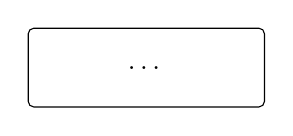
\begin{tikzpicture}
        \node[draw,rounded corners=2pt,minimum width=3cm,minimum height=1cm] {\ldots};
    \end{tikzpicture}}\only<handout:2|13->{\downsize{.4\linewidth}{\begin{tikzpicture}[baseline=-17.5ex,every node/.append style={outer sep=3pt}]
        % indices
    \def\c{\multicolumn{1}{c|}}\def\cc{\multicolumn{1}{|c|}}\tabcolsep=.45cm\def\arraystretch{1.5}
    \onslide<13->{\node[right] (a) at (0,0) {\begin{tabular}{r*7c}
        \llap{Index:} & 0 & 1 & 2 & 3 & 4 & 5 & 6 \\
        \cline{2-8}
        \llap{Array:} & \cc1 & \c3 & \c4 & \c6 & \c7 & \c{10} & \c{13} \\
        \cline{2-8}
    \end{tabular}};}
    \onslide<14->{\node[below left,yshift=-.25cm] (b) at (a.south east) {\begin{tabular}{|*3{c|}}
        \hline 7 & 10 & 13 \\ \hline
    \end{tabular}};
    \draw[-Kite] ([xshift=2mm]a.south) |- (b.west) node[left,pos=.275] {\(k > 6\)};}
    \onslide<15->{\node[below right,yshift=-.25cm] (c) at (b.south west) {\begin{tabular}{|c|}
        \hline 7 \\ \hline
    \end{tabular}};\draw[-Kite] (b.south) |- (c.east) node[right,pos=.275] {\(k < 10\)};}
    \onslide<16->{\node[below=.5cm] (d) at (c.south) {index(7) = 4};
    \draw[-Kite] (c) to[edge node={node[left] {\(k = 7\)}}](d);}
    \onslide<13->{\node[above right,yshift=2cm] at(current bounding box.south west) {Die Suche nach der \(7\).};}
\end{tikzpicture}}}}\only<handout:1|-12>{\vspace*{-.2\baselineskip}}\only<handout:2|13->{\vspace*{-.7\baselineskip}}
\end{center}
        \onslide<1->
    \end{aufgabe}
\begin{tikzpicture}[overlay, remember picture]
    \onslide<handout:1|11>{\node[above left=-1.5cm] at (current page.south east) {\rotatebox{30}{\usebox\sadGrapplePingu}};}
    \foreach[count=\i] \l in {12,...,15} {
        \onslide<handout:0|\l>{\node[above left=-1.5cm-\i*.25cm] at (current page.south east) {\rotatebox{30}{\usebox\sadGrapplePingu}};}
    }
    \onslide<handout:2|16->{\node[above left=-1.5cm-5*.25cm] at (current page.south east) {\rotatebox{30}{\usebox\sadGrapplePingu}};}
\end{tikzpicture}
\end{frame}
\MakeThePinguExplainIt[text width=5.35cm]{cap=!hide,glasses=!hide,cup=cprimary,right item angle=-10}{\hbox{1.~Basisfall:} keine Elemente mehr.\\\hbox{2.~Basisfall:} Element gefunden.\\Sonst: Suche links/rechts.}
\begin{frame}[c]{Präsenzaufgabe - Lösung}
\begin{itemize}[<+(1)->]
    \itemsep15.5pt
    \item Wir erschaffen eine Suche: \only<2->{\textattachfile{\curpath BinarySearch.java}{BinarySearch.java}}. \info{Eine binäre Suche}
    \item Die Idee: \begin{itemize}
        \item Wir markieren das zu durchsuchende Fenster mit \bjava{left} und \bjava{right}.\hfill \raisebox{-.15\height}{\tikz{\foreach[count=\i] \a in {lightgray, lightgray, shadeA, shadeA, shadeA, shadeA, lightgray} {\node[circle,fill=\a] (\i) at (\i/2,0) {};}\pgfinterruptboundingbox\node[above=-.6mm] at(3.north) {\scriptsize\strut\T{left}}; \node[above=-.6mm] at(6.north) {\scriptsize\strut\T{right}}; \node[above=-.9mm,lightgray,scale=.65] at(3.north) {\faCaretDown}; \node[above=-.9mm,lightgray,scale=.65] at(6.north) {\faCaretDown};\endpgfinterruptboundingbox}}
        \item Ist das Fenster leer, haben wir das Element nicht gefunden.%\hfill \T{right < left}
        \item Sonst prüfen wir: Ist das mittlere Element das Gesuchte?
        \item Ist es kleiner, suchen wir links, ist es größer, rechts weiter.
    \end{itemize}
    \item Dafür nutzen wir die Hilfsmethode: \bjava{binarySearch(int[] array, int left, int right, int element)}.
    \item Wir beginnen mit der Suche im gesamten Array: \bjava{binarySearch(array, 0, array.length - 1, element);}
\end{itemize}
\begin{tikzpicture}[overlay, remember picture]
    \onslide<10->{\node[left=-9.5mm,scale=.8] at(current page.-11.35) {\usebox\pinguexplainbox};}
\end{tikzpicture}%
\end{frame}

\begin{frame}[fragile]{Präsenzaufgabe - Lösung}
\SetupLstHl\lstfs{10}
\begin{plainjava}
!*\onslide<2->*!|ihl|static int binarySearch(int[] array, int left, int right, int element) {|ihl|
!*\onslide<3->*!    // !*\textbf{\solGet{comments}{1)}}*! Fenster ist leer
!*\onslide<4->*!    if(right < left)
!*\onslide<4->*!        return -1;
!*\onslide<2->*!
!*\onslide<5->*!    int middle = left + (right - left) / 2;
!*\onslide<3->*!    // !*\textbf{\solGet{comments}{2)}}*! Ist das Mittlere das Gesuchte?
!*\onslide<6->*!    if(array[middle] == element)
!*\onslide<6->*!        return middle;
!*\onslide<3->*!    // !*\textbf{\solGet{comments}{3)}}*! Kleiner: suche links weiter
!*\onslide<7->*!    else if(array[middle] > element)
!*\onslide<7->*!        return binarySearch(array, left, middle - 1, element);
!*\onslide<3->*!    // !*\textbf{\solGet{comments}{4)}}*! Größer: suche rechts weiter
!*\onslide<8->*!    else
!*\onslide<8->*!        return binarySearch(array, middle + 1, right, element);
!*\onslide<2->*!|ihl|}|ihl|
\end{plainjava}
\end{frame}


\begin{frame}[fragile]{Präsenzaufgabe - Lösung}
\begin{itemize}[<+(1)->]
    \itemsep6.5pt
    \item Einen Teil haben wir noch nicht gemacht:\pause \begin{center}
        \parbox{.725\linewidth}{\textcolor{gray}{Sollte das Elemente mehrfach vorhanden sein, soll der kleinste Index zurückgegeben werden}}
    \end{center}
    \item Idee: Wir verringern den Index, solange das Element immer noch das Gesuchte ist:
\SetupLstHl\lstfs{10}\begin{plainjava}
!*\onslide<5->*!public static int find(int[] array, int element) {
!*\onslide<6->*!    int index = binarySearch(array, 0, array.length - 1, element);
!*\onslide<7->*!    if(index == -1) return -1;
!*\onslide<5->*!
!*\onslide<8->*!    for(int i = 1; i <= index; i++) {
!*\onslide<9->*!        if(array[index - i] != element)
!*\onslide<9->*!            return index - i + 1;
!*\onslide<8->*!    }
!*\onslide<10->*!    return 0;
!*\onslide<5->*!}
\end{plainjava}
\end{itemize}
\begin{tikzpicture}[overlay, remember picture]
    \begin{uncoverenv}<11->
    \node[above left=.25cm,text width=10cm,scale=.5,xshift=-.5cm,yshift=1.25cm,draw=gray,thick,rounded corners=2pt] at(current page.south east) (a) {\begin{plainjava}[aboveskip=0pt,belowskip=0pt]
// return findLower(array, element, index, 1);
int findLower(int[] arr, int e, int idx, int i) {
    if(i > idx)
        return 0;
    if (arr[idx - i] != e)
        return idx - i + 1;
    return findLower(arr, e, idx, i + 1);
}
    \end{plainjava}};
    \node[above right,gray] at(a.north west) {\footnotesize Rekursive Variante\quad\tiny (etwas zu lang)};
\end{uncoverenv}
\end{tikzpicture}
\end{frame}

\iffull
\newsavebox\pinguBSa \savebox\pinguBSa{\PinguBanner{-14}{strawhat}}
\newsavebox\pinguBSaa \savebox\pinguBSaa{\PinguBanner{-14}{cloak=pingu@black}}
\newsavebox\pinguBSb \savebox\pinguBSb{\PinguBanner{24}{hat,hat position={1:(0cm,-.09cm){1.33}}}}
\newsavebox\pinguBSbb \savebox\pinguBSbb{\PinguBanner{24}{cake-hat}}
\newsavebox\pinguBSc \savebox\pinguBSc{\PinguBanner{42}{halo}}
\newsavebox\pinguBSd \savebox\pinguBSd{\PinguBanner{109}{headband,pants}}
\newsavebox\pinguBSe \savebox\pinguBSe{\PinguBanner{113}{vr-headset}}
\newcommand<>\PinguBS[2]{$\underset{\onslide#3{\text{\huge\strut\T{#1}}}}{\expandafter\usebox\csname pinguBS#2\endcsname}$}
\begin{frame}[fragile]{Präsenzaufgabe - Lösung\hfill Statische Simulation\llap{\smash{\raisebox{-.3\baselineskip}{\scalebox{.7}{\itshape\tiny \say{Statische},\;weil\;ich\;keinen\;Platz\;mehr\;für\;static\;hatte\;:D}}}}}
\SetupLstHl\lstfs{8}\vspace*{-.5\baselineskip}\begin{columns}[c,onlytextwidth]
\column{.495\linewidth}
\begin{plainjava}
!*\onslide<2->*!!*\md[1]{7,13}*!int search(int[] arr, int l, int r, int e) {
!*\onslide<2->*!  !*\md{8,14}*!if(r < l) return -1; !*\rBS<handout:2|8-12>{r=6, l=0}\rBS<handout:3|14-17>{r=2, l=0}*!
!*\onslide<2->*!  !*\md{9,15}*!int mid = l + (r - l) / 2; !*\rBS<handout:2|9-12>{mid=3}\rBS<handout:3|15-17>{mid=1}*!
!*\onslide<2->*!  !*\md[3]{10,16}*!if (arr[mid] == e) return m!*\mb{17}*!id; !*\rBS<handout:2|10-12>{e=-14}\rBS<handout:3|16-17>{e=-14, mid=1}*!
!*\onslide<2->*!  !*\md{11}*!else if (arr[mid] > e) !*\rBS<handout:2|11-12>{24 > -14}*!
!*\onslide<2->*!      !*\md[2]{12}\mg[3]{13-17}*!return search(arr, l, mid - 1, e);!*\ml{18}*!
!*\onslide<2->*!  else
!*\onslide<2->*!      return search(arr, mid + 1, r, e);
!*\onslide<2->*!}!*\ml{19}*!

!*\onslide<3->*!!*\md5*!int find(int[] arr, int e) {
!*\onslide<3->*!  !*\md{6}\mg[1-3]{7-19}*!int idx = search(arr, 0, arr.length - 1, e);!*\ml{20}*!
!*\onslide<3->*!  !*\md[4]{21}*!if(idx == -1) return -1; !*\rBS<handout:4|21-25>{idx=1}*!
!*\onslide<3->*!  !*\md{22,24}*!for(int i = 1; i <= idx; i++) { !*\rBS<handout:0|22-23>{i=1, 1<=1}\rBS<handout:0|24-25>{i=2, 2<=1}*!
!*\onslide<3->*!      !*\md{23}*!if(arr[idx - i] != e) !*\rBS<handout:0|23>{arr[0]=-14, e=-14}*!
!*\onslide<3->*!          return idx - i + 1;
!*\onslide<3->*!  }
!*\onslide<3->*!  !*\md{25}*!return 0; !*\onslide<handout:5|25->*!//Wir sind ganz links
!*\onslide<3->*!}
\end{plainjava}
\column{.505\linewidth}
\centering\onslide<handout:1-|4->{\begin{tikzpicture}
\only<handout:3-|13-19>{\scope[transparency group,opacity=.6]}
\only<handout:4-|20->{\scope[transparency group,opacity=.3]}
    \node at (0,0) {\downsize\linewidth{\PinguBS<handout:2-|7->{left}{a}~\PinguBS{}{aa}~\PinguBS{}b~\PinguBS<handout:2-|9->{mid}{bb}~\PinguBS{}c~\PinguBS{}d~\PinguBS<handout:2-|7->{right}e}};
\only<handout:4-|20->{\endscope}
\only<handout:3-|13-19>{\endscope}
\end{tikzpicture}}\bigskip\par
\only<handout:3-|13->{\begin{tikzpicture}
    \only<handout:4-|20->{\scope[transparency group,opacity=.6]}
    \node at (0,0) {\downsize\linewidth{\PinguBS<13->{left}{a}~\PinguBS<15->{mid}{aa}~\PinguBS<13->{right}b~\PinguBS{}{bb}~\PinguBS{}c~\PinguBS{}d~\PinguBS<7->{}e}};
    \only<handout:4-|20->{\endscope}
\end{tikzpicture}}\bigskip\par
\only<handout:4-|20->{\begin{tikzpicture}
    \node at (0,0) {\downsize\linewidth{\PinguBS{}{a}~\PinguBS<20->{idx}{aa}~\PinguBS{}b~\PinguBS{}{bb}~\PinguBS{}c~\PinguBS{}d~\PinguBS<7->{}e}};
\end{tikzpicture}}
\end{columns}\vspace*{-1.15\baselineskip}
\begin{center}
    \footnotesize\onslide<4->{\mbox{\md[0]{4}\mg[1-3]{5-25}\bjava{find(|ihl|new int[]\{-14, -14, 24, 24, 42, 109, 113\}|ihl|, -14);}}}\ml[5]{26}\smash{~~~~\onslide<handout:5|26->{~\bjava{// :yields: 0}}}
\end{center}
\end{frame}

\newsavebox\pinguTalkHSa \savebox\pinguTalkHSa{\tikz\pingu[eyes=wink, left wing wave, right wing grab,bow tie=paletteA];}
\newsavebox\pinguTalkHSb \savebox\pinguTalkHSb{\tikz\pingu[eyes=wink, left wing wave, right wing grab,tie=paletteB,shirt=pingu@red!60!pingu@black!60!pingu@white,second shirt=pingu@black,shirt above,princess crown];}
\begin{frame}[fragile]{Präsenzaufgabe - Lösung\hfill Stackische Heap-Simulation}
\vspace*{-.5\baselineskip}\begin{columns}[c,onlytextwidth]
\column{.495\linewidth}\SetupLstHl\lstfs{8}
\begin{plainjava}
!*\onslide<2->*!!*\md[1]{7,13}*!int search(int[] arr, int l, int r, int e) {
!*\onslide<2->*!  !*\md{8,14}*!if(r < l) return -1; !*\rBS<handout:2|8-12>{r=6, l=0}\rBS<handout:3|14-17>{r=2, l=0}*!
!*\onslide<2->*!  !*\md{9,15}*!int mid = l + (r - l) / 2; !*\rBS<handout:2|9-12>{mid=3}\rBS<handout:3|15-17>{mid=1}*!
!*\onslide<2->*!  !*\md[3]{10,16}*!if (arr[mid] == e) return m!*\mb{17}*!id; !*\rBS<handout:2|10-12>{e=-14}\rBS<handout:3|16-17>{e=-14, mid=1}*!
!*\onslide<2->*!  !*\md{11}*!else if (arr[mid] > e) !*\rBS<handout:2|11-12>{24 > -14}*!
!*\onslide<2->*!      !*\md[2]{12}\mg[3]{13-17}*!return search(arr, l, mid - 1, e);!*\ml{18}*!
!*\onslide<2->*!  else
!*\onslide<2->*!      return search(arr, mid + 1, r, e);
!*\onslide<2->*!}!*\ml{19}*!

!*\onslide<3->*!!*\md5*!int find(int[] arr, int e) {
!*\onslide<3->*!  !*\md{6}\mg[1-3]{7-19}*!int idx = search(arr, 0, arr.length - 1, e);!*\ml{20}*!
!*\onslide<3->*!  !*\md[4]{21}*!if(idx == -1) return -1; !*\rBS<handout:4|21-25>{idx=1}*!
!*\onslide<3->*!  !*\md{22,24}*!for(int i = 1; i <= idx; i++) { !*\rBS<handout:0|22-23>{i=1, 1<=1}\rBS<handout:0|24-25>{i=2, 2<=1}*!
!*\onslide<3->*!      !*\md{23}*!if(arr[idx - i] != e) !*\rBS<handout:0|23>{arr[0]=-14, e=-14}*!
!*\onslide<3->*!          return idx - i + 1;
!*\onslide<3->*!  }
!*\onslide<3->*!  !*\md{25}*!return 0; !*\onslide<handout:5|25->*!//Wir sind ganz links
!*\onslide<3->*!}
\end{plainjava}
\column{.505\linewidth}
\raggedleft\makeatletter
\lhns@elemwidth4.5cm
\lhns@minborderheight11cm
\makeatother
\onslide<5->{\raisebox{.55cm}{\downsizeBoth{5.85cm}\linewidth{\begin{tikzpicture}[lhns@basestyle/.append style={execute at begin node=\strut,font=\ttfamily},lhns@blockstyle/.append style={draw=gray,thick}]
\begin{heap-n-stack}{}
\heap{\bjava{\{-14, :ldots:, 114\}}}
\renderheap

\stack{\textbf{main}}
\stack{$\ldots$}
\only<handout:5-|26->{\stack{\say{\bjava{find = 0}}}}
\only<handout:1-4|-25>{\stack{\textbf{find}}
\stack{arr}
\stack{\bjava{e = -14}}
\only<handout:1-3|6-19>{\stack{\bjava{idx =}~\textcolor{gray}{?}}}
\only<handout:4|20->{\stack{\bjava{idx = 1}}}
\only<handout:0|22-23>{\stack{\bjava{i = 1}}}
\only<handout:0|24>{\stack{\bjava{i = 2}}}
\only<handout:1-3|7-18>{\stack{\textbf{search}}
\only<handout:1-2|-12>{\stack{arr}
\stack{\bjava{l = 0}}
\stack{\bjava{r = 6}}
\stack{\bjava{e = -14}}}
}
\only<handout:2|9-12>{\stack{\bjava{mid = 3}}}
\only<handout:3|13-17>{\stack{$\ldots$}
\stack{\textbf{search}}
\stack{arr}
\stack{\bjava{l = 0}}
\stack{\bjava{r = 2}}
\stack{\bjava{e = -14}}
}
\only<handout:3|15-17>{\stack{\bjava{mid = 1}}}
\only<handout:5|18>{\stack{$\ldots$}\stack{\say{\bjava{search = 1}}}}
\only<handout:5|19>{\stack{\say{\bjava{search = 1}}}}}
\renderstack
\only<-25>{
\only<handout:1-4>{\draw[lhns] (stack-3.east) to[out=20,in=220] (heap-0.west);}
\only<handout:1-3|7-18>{
    \draw[lhns] (stack-7.east) to[out=35,in=220] (heap-0.west);
}
\only<handout:3|13-17>{
    \draw[lhns] (stack-9.east) to[out=37,in=218] (heap-0.west);
}}
\end{heap-n-stack}
\end{tikzpicture}}}}~~
\end{columns}\vspace*{-1\baselineskip}
\begin{center}\SetupLstHl\lstfs{8}
    \footnotesize\onslide<4->{\mbox{\md[0]{4}\mg[1-3]{5-25}\bjava{find(|ihl|new int[]\{-14, -14, 24, 24, 42, 109, 113\}|ihl|, -14);}}}\ml[5]{26}\smash{~~~~\onslide<handout:5|26->{~\bjava{// :yields: 0}}}
\end{center}
\begin{tikzpicture}[overlay,remember picture]
    \onslide<handout:1|6>{%
        \node[left=-.95cm,scale=.6] (pingu) at ([yshift=-1.5cm]current page.east) {\rotatebox[origin=c]{70}{\usebox\pinguTalkHSa}};
        \node[above left,scale=.6,text width=4.425cm,align=right,xshift=-1cm,yshift=-.325cm] at (pingu.north) {Dabei muss der \bjava{find(int[], int)}-\\Aufruf nicht \hbox{direkt} in \bjava{main} sein.};
    }
    \onslide<handout:3|13>{%
        \node[left=-.95cm,scale=.6] (pingu) at ([yshift=-1.5cm]current page.east) {\rotatebox[origin=c]{70}{\usebox\pinguTalkHSb}};
        \node[above left,scale=.6,text width=4.425cm,align=right,xshift=-.665cm,yshift=-.325cm] at (pingu.north) {Genau genommen wird da (in \bjava{...}) noch mehr abgelegt. Zum Beispiel, wo es in der aufrufenden Methode weitergeht)\ldots};
    }
\end{tikzpicture}%
\end{frame}
\fi


\section{Übungsblatt 9}
\subsection{Aufgabe 1}
\iffull
\begin{frame}[c,fragile]{Übungsblatt 9 - Aufgabe 1}
    \onslide<2->{\only<3->{\color{gray}}In dieser Aufgabe sollen Sie eine Methode implementieren, welche die Summe errechnet die ein Startkapital in einer bestimmten Anzahl an Jahren mit einem fixen Jahreszinssatz erreicht. Die Methode soll die folgende \only<handout:0|-2>{Signatur}\only<3->{\cancel{Signatur} Gestalt} haben:
    {\color{black}\bjava{public static double compoundInterest(double capital, double interestRate, int years)}}
    Hierbei soll der Parameter \texttt{capital} das Startkapital angeben, \texttt{interestRate} den Zinssatz in Prozent und \texttt{years} die Laufzeit.
    Verwenden Sie bei ihrer Implementierung {\color{black}keine Schleifen}, sondern {\color{black}rekursive Methoden-Aufrufe}!}\color{black}\bigskip

    \lstfs{10}\onslide<4->{Iterativer Ansatz:}
\begin{columns}[c,onlytextwidth]
\column{.5\linewidth}
\begin{plainjava}
!*\onslide<5->*!for(int i = 0; i < years; i++) {
!*\onslide<6->*!    capital *= (1 + interestRate);
!*\onslide<5->*!}
\end{plainjava}
\column{.5\linewidth}
\begin{plainjava}
!*\onslide<7->*!for(int i = years; i > 0; i--) {
!*\onslide<8->*!    capital *= (1 + interestRate);
!*\onslide<7->*!}
\end{plainjava}
\end{columns}
\end{frame}
\fi

\MakeThePinguExplainIt[text width=12cm]{cap=!hide,headphones,glasses=!hide,eyes wink,cup=!hide,heart=shadeA,silver medal,right item angle=-56}{Warum die herunterzählende Variante? Nun, sie spart uns eine weitere Variable in der Rekursion. So müssen wir nur prüfen, wann \bjava{years} den Wert \bjava{0} erreicht. Andernfalls wäre eine weitere Variable notwendig um das ursprüngliche \bjava{years} zu halten.}
\begin{frame}[t,fragile]{Übungsblatt 9 - Aufgabe 1}
    \begin{itemize}[<+(1)->]
        \item Die Datei befindet sich hier: \only<2->{\textattachfile{\curpath CompoundInterest.java}{CompoundInterest.java}}
    \end{itemize}\vfill
\SetupLstHl\lstfs{10}%
\begin{plainjava}
!*\onslide<3->*!|ihl|public static|ihl|
!*\onslide<3->*!double compoundInterest(double capital, double interestRate, int years) {
!*\onslide<4->*!    if(years == 0)
!*\onslide<5->*!        return capital;
!*\onslide<4->*!    else
!*\onslide<6->*!        return compoundInterest(capital * (1 + interestRate), interestRate,
!*\onslide<6->*!            years - 1);
!*\onslide<3->*!}
\end{plainjava}
\vfill\null
\begin{tikzpicture}[overlay,remember picture]
    \node[below left=.35cm,yshift=-1.5cm,text width=6.5cm,scale=.6,draw=gray,thick,rounded corners=2pt] at(current page.north east) {%
\begin{plainjava}[aboveskip=0pt,belowskip=0pt]
for(int i = years; i > 0; i--) {
    capital *= (1 + interestRate);
}
\end{plainjava}
    };
\onslide<7->{\node[left=-7mm,scale=.8] at(current page.-24) {\usebox\pinguexplainbox};}
\end{tikzpicture}
\end{frame}

\subsection{Aufgabe 2}
\iffull
\begin{frame}[c,fragile]{Übungsblatt 9 - Aufgabe 2}
    \onslide<2->{\only<3->{\color{gray}}In dieser Aufgabe sollen Sie die Methode {\color{black}\bjava{public static boolean isPalindrome} \bjava{(String s)}} implementieren, welche überprüfen soll ob es sich bei dem als Parameter übergebenen String \bjava{s} um ein Palindrom handelt. Ein Palindrom ist ein Wort, das vorwärts und rückwärts gelesen identisch ist. Die Überprüfung soll {\color{black}nicht case-sensitive} sein, d.h. das Wort \textit{Kajak} soll zum Beispiel ein gültiges Palindrom sein.
    Verwenden Sie bei ihrer Implementierung {\color{black}keine Schleifen}, sondern {\color{black}rekursive Methoden-Aufrufe!}}\bigskip

    \onslide<4->{\color{black}Idee:}
    \footnotesize\begin{itemize}
        \item<5-> Prüfe für \(i = 0\) bis \(i = \floor{\sfrac{\text{\bjava{s.length}}}{2}}\), ob \say{\bjava{s[i] == s[s.length - i - 1]}}.
        \item<6-> \bjava{String::toLowerCase()} entweder für jeden Vergleich oder einmal per Hilfsmethode.
        \item<7-> Noch einfacher: Anstelle \bjava{i} zu inkrementieren, löschen wir das erste und letzte Zeichen nach dem Vergleich (via \bjava{String::substring(int, int)}---das Ende ist exklusiv)!
    \end{itemize}
\end{frame}
\fi

\begin{frame}[fragile]{Übungsblatt 9 - Aufgabe 2}
    \begin{itemize}[<+(1)->]
        \item Die Datei befindet sich hier: \only<2->{\textattachfile{\curpath Palindrome.java}{Palindrome.java}}
    \end{itemize}\vfill
\SetupLstHl\lstfs{10}%
\begin{plainjava}
!*\onslide<3->*!public static boolean isPalindrome(String s) { // die "Hilfsmethode"
!*\onslide<4->*!    return isPalindromeRecursive(s.toLowerCase());
!*\onslide<3->*!}


!*\onslide<5->*!private static boolean isPalindromeRecursive(String s) {
!*\onslide<6->*!    if(s.length() < 2) // Basisfall: weniger als zwei Zeichen (Abrunden)
!*\onslide<6->*!        return true;
!*\onslide<7->*!    else if(s.charAt(0) != s.charAt(s.length() - 1)) // Basisfall
!*\onslide<7->*!        return false;
!*\onslide<8->*!    else // Rekursionsfall
!*\onslide<8->*!        return isPalindromeRecursive(s.substring(1, s.length() - 1));
!*\onslide<5->*!}
\end{plainjava}
\vfill\null
\end{frame}

\iffull
\MakeThePinguExplainIt[text width=7cm]{cap=!hide,glasses=!hide,sunglasses round,eyes shiny,cup=!hide,santa beard,santa hat,right item angle=-142,staff right length=17mm}{Mit \bjava{:lan:ret:c:urn:ran:} haben wir hier die zurückzugebenden anonymen Variablen referenziert. Generell ist hier das \say{Speichern} der Position für den Aufstieg der Rekursion informal dargestellt.}
\begin{frame}[c,fragile]{Übungsblatt 9 - Aufgabe 2\hfill Sie Simulantario Sie!}
\SetupLstHl\lstfs{10}\begin{plainjava}
!*\onslide<2->*!!*\md4*!private static boolean isPalindrome(String s) { !*\rBS<handout:2-4|4->{s=\dq RegalelaGEr\dq }*!
!*\onslide<2->*!    !*\md5*!return isPalindrom!*\mb{7,38}\mbg[2-3]{8-42}*!eRecursive(s!*\mb6*!.toLowerCase());!*\ml[4]{43}*! !*\rBS<handout:2-3|6-41>{\dq regalelager\dq }~~\rBS<handout:4|43>{true}*!
!*\onslide<2->*!}
!*\onslide<2->*!!*\md{8,15,20,25,30,35}*!private static boolean isPalindromeRecursive(String s) { !*\rBS<handout:0|8-14>{s=\dq regalelager\dq }\rBS<handout:0|15-19>{s=\dq egalelage\dq }\rBS<handout:0|20-24>{s=\dq galelag\dq }\rBS<handout:2-3|25-29>{s=\dq alela\dq }\rBS<handout:0|30-34>{s=\dq lel\dq }\rBS<handout:0|35-37>{s=\dq e\dq }*!
!*\onslide<2->*!    !*\md{9,16,21,26,31,36}*!if(s.length() < 2) return true;!*\ml[3]{37}*!
!*\onslide<2->*!    !*\md[2]{10,17,22,27,32}*!else if(s.charAt(0) != s.charAt(s.length() - 1)) return false; !*\rBS<handout:0|10-14>{'r'!='r'}\rBS<handout:0|17-19>{'e'!='e'}\rBS<handout:0|22-24>{'g'!='g'}\rBS<handout:2|27-29>{'a'!='a'}\rBS<handout:0|32-34>{'l'!='l'}*!
!*\onslide<2->*!    !*\md{11,18,23,28,33}*!else return isPalindrom!*\mb{14,19,24,29,34}\mbg[2-3]{15-18,20-23,25-28,30-33,35-41}*!eRecursive(s!*\mb{13}*!.substring(1, s!*\mb{12}*!.length() - 1));!*\ml{38,39,40,41,42}*!
!*\onslide<2->*!}
\end{plainjava}
\only<handout:1|3>{\begin{center}
    \huge\bfseries \say{RegalelaGEr}\\[-2mm]
    {\normalfont\info{Wer sieht auch ein \T{e}, dass die Arme hochwirft?}}
\end{center}}
\begin{onlyenv}<handout:2-4|4-43>\begin{center}\lstfs{6}\lstset{aboveskip=0pt,belowskip=0pt,add to literate={:ll:}{{{\color{lightgray!60!gray}$\ldots$}}}1}
    \begin{tikzpicture}[b/.style={draw=gray,fill=white,text width=4.1cm,minimum height=2.25cm,thick,rounded corners=2pt,inner xsep=1em}]
            \node[b] (a) at(0,0) {%
\begin{plainjava}
!*\md4*!boolean isPalindrome(String s) {
    !*\md5*!return isPalindrom!*\mb[1-]{7-42}*!eRecurs!*\mb{6}*!:ll:!*\ml{43-}*!
}
\end{plainjava}\medskip
\centerline{\bjava{s = "RegalelaGEr"}\onslide<43->{ \bjava{:lan:ret:c:urn:ran: = true}}}
            };
\node[above right,gray] at(a.south west) {\(1\)};
\begin{onlyenv}<handout:-3|8-42>\node[b,right=-4cm,yshift=-.1cm] (b) at(a.east) {%
\begin{plainjava}
!*\md8*!boolean isPalindromeRecursive:ll:
    !*\md9*!if(s.length() < 2) return:ll:
    !*\md{10}*!else if(s.charAt(0) != s.c:ll:
    !*\md{11}*!else return isPalindrom!*\mb[1-]{14-41}*!eRe!*\mb{12-13}*!:ll:!*\ml{42-}*!
}
\end{plainjava}\medskip
\centerline{\bjava{s = "regalelager"}\onslide<42->{ \bjava{:lan:ret:c:urn:ran: = true}}}
        };
\node[above right,gray] at(b.south west) {\(2\)};
    \end{onlyenv}
\begin{onlyenv}<handout:-3|15-41>\node[b,right=-4cm,yshift=-.1cm] (c) at(b.east) {%
\begin{plainjava}
!*\md{15}*!boolean isPalindromeRecursive:ll:
    !*\md{16}*!if(s.length() < 2) return:ll:
    !*\md{17}*!else if(s.charAt(0) != s.c:ll:
    !*\md{18}*!else return isPalindrom!*\mb[1-]{19-40}*!eRe:ll:!*\ml{41-}*!
}
\end{plainjava}\medskip
\centerline{\bjava{s = "egalelage"}\onslide<41->{ \bjava{:lan:ret:c:urn:ran: = true}}}
        };
\node[above right,gray] at(c.south west) {\(3\)};
    \end{onlyenv}
\begin{onlyenv}<handout:-3|20-40>\node[b,right=-4cm,yshift=-.1cm] (d) at(c.east) {%
\begin{plainjava}
!*\md{20}*!boolean isPalindromeRecursive:ll:
    !*\md{21}*!if(s.length() < 2) return:ll:
    !*\md{22}*!else if(s.charAt(0) != s.c:ll:
    !*\md{23}*!else return isPalindrom!*\mb[1-]{24-39}*!eRe:ll:!*\ml{40-}*!
}
\end{plainjava}\medskip
\centerline{\bjava{s = "galelag"}\onslide<40->{ \bjava{:lan:ret:c:urn:ran: = true}}}
        };
    \node[above right,gray] at(d.south west) {\(4\)};
    \end{onlyenv}
\begin{onlyenv}<handout:-3|25-39>\node[b,right=-4cm,yshift=-.1cm] (e) at(d.east) {%
\begin{plainjava}
!*\md{25}*!boolean isPalindromeRecursive:ll:
    !*\md{26}*!if(s.length() < 2) return:ll:
    !*\md{27}*!else if(s.charAt(0) != s.c:ll:
    !*\md{28}*!else return isPalindrom!*\mb[1-]{29-38}*!eRe:ll:!*\ml{39-}*!
}
\end{plainjava}\medskip
\centerline{\bjava{s = "alela"}\onslide<39->{ \bjava{:lan:ret:c:urn:ran: = true}}}
        };
\node[above right,gray] at(e.south west) {\(5\)};
    \end{onlyenv}
\begin{onlyenv}<handout:3|30-38>\node[b,right=-4cm,yshift=-.1cm] (f) at(e.east) {%
\begin{plainjava}
!*\md{30}*!boolean isPalindromeRecursive:ll:
    !*\md{31}*!if(s.length() < 2) return:ll:
    !*\md{32}*!else if(s.charAt(0) != s.c:ll:
    !*\md{33}*!else return isPalindrom!*\mb[1-]{34-37}*!eRe:ll:!*\ml{38-}*!
}
\end{plainjava}\medskip
\centerline{\bjava{s = "lel"}\onslide<38->{ \bjava{:lan:ret:c:urn:ran: = true}}}
        };
\node[above right,gray] at(f.south west) {\(6\)};
    \end{onlyenv}
\begin{onlyenv}<handout:3|35-37>\node[b,right=-4cm,yshift=-.1cm] (g) at(f.east) {%
\begin{plainjava}
!*\md{35}*!boolean isPalindromeRecursive:ll:
    !*\md{36}*!if(s.length() < 2) return:ll:!*\ml[1-]{37-}*!
    else if(s.charAt(0) != s.c:ll:
    else return isPalindromeRe:ll:
}
\end{plainjava}\medskip
\centerline{\bjava{s = "e"}\onslide<37->{ \bjava{:lan:ret:c:urn:ran: = true}}}
        };
\node[above right,gray] at(g.south west) {\(7\)};
    \end{onlyenv}
    \end{tikzpicture}
\end{center}
\end{onlyenv}
\begin{tikzpicture}[remember picture,overlay]
    \onslide<handout:4-|44->{\node[left=-7mm,scale=.8] at(current page.-20) {\usebox\pinguexplainbox};}
\end{tikzpicture}
\end{frame}
\fi

\iffull
\begin{frame}[c,fragile]{Übungsblatt 9 - Aufgabe 2\hfill Iterativer Ansatz}
    \begin{itemize}[<+(1)->]
        \item Die ersten beiden Aufgaben lassen sich \textit{einfacher} Iterativ prüfen.
        \item Für das Palindrom schauen wir für jedes Zeichen \(i\) der \say{linken Hälfte} ob es mit dem gespiegelten \(\text{\T{length}} - i - 1\) der \say{rechten Hälfte} übereinstimmt:
    \end{itemize}
\begin{plainjava}
!*\onslide<4->*!public static boolean isPalindromeIterative(String s) {
!*\onslide<5->*!    s = s.toLowerCase();
!*\onslide<6->*!    for(int i = 0; i < s.length() / 2; i++) {
!*\onslide<7->*!        if(s.charAt(i) != s.charAt(s.length() - i - 1))
!*\onslide<7->*!            return false;
!*\onslide<6->*!    }
!*\onslide<8->*!    return true;
!*\onslide<4->*!}
\end{plainjava}
\end{frame}

\begin{frame}[c,fragile]{Übungsblatt 9 - Aufgabe 2\hfill Iterativer Ansatz, II}
    \lstfs{10}\begin{itemize}[<+(1)->]
        \item Dies können wir als Tail-Rekursion umschreiben (\only<2->{\textattachfile{\curpath PalindromeIterative.java}{PalindromeIterative.java}}):
    \end{itemize}
\begin{plainjava}
!*\onslide<3->*!public static boolean isPalindrome(String s) {
!*\onslide<4->*!    return helper(s.toLowerCase(), 0);
!*\onslide<3->*!}
!*\onslide<3->*!
!*\onslide<5->*!private static boolean helper(String s, int i) {
!*\onslide<6->*!    if (i >= s.length() / 2)
!*\onslide<6->*!        return true;
!*\onslide<7->*!    if (s.charAt(i) != s.charAt(s.length() - i - 1))
!*\onslide<7->*!        return false;
!*\onslide<8->*!    return helper(s, i + 1);
!*\onslide<5->*!}
\end{plainjava}
\begin{tikzpicture}[overlay, remember picture]
\begin{uncoverenv}<9->
    \node[above left=.925cm,text width=9.65cm,draw=gray,thick,rounded corners=2pt,scale=.65,yshift=.25cm] at(current page.south east) {%
\begin{plainjava}[aboveskip=0pt, belowskip=0pt]
s = s.toLowerCase();
for(int i = 0; i < s.length() / 2; i++) {
    if(s.charAt(i) != s.charAt(s.length() - i - 1))
        return false;
}
return true;
\end{plainjava}
    };
\end{uncoverenv}
\end{tikzpicture}
\end{frame}
\fi

\subsection{Aufgabe 3}
\iffull
\begin{frame}[c,fragile]{Übungsblatt 9 - Aufgabe 3}
    \onslide<2->{\only<3->{\color{gray}}In dieser Aufgabe sollen Sie die Methode {\color{black}\bjava{public static void printCombinations} \bjava{(int[] array, int n)}} implementieren, welche ein Integer Array und eine natürliche Zahl \bjava{n} als Parameter übernimmt. Die Methode soll rekursiv alle möglichen Kombinationen aus \bjava{n} Elementen des Arrays ausgeben. Hierbei soll \bjava{n} maximal so groß sein wie die Länge des Arrays.
    Verwenden Sie bei ihrer Implementierung {\color{black}rekursive Methoden-Aufrufe} wann immer möglich.
    Sie benötigen {\color{black}maximal eine Schleife} für die Lösung.\bigskip\par
    Hinweis: Sie können sich entscheiden ob Sie die Ausgabe der Kombinationen mit oder ohne Wiederholung von Elementen implementieren.}
\end{frame}
\fi

\MakeThePinguExplainIt[text width=9cm]{cap=!hide,glasses=!hide,cloak=pingu@black,eyes shiny,right item angle=33,rotate=10}{Da wir die Maximalgröße der Ausgabekombinationen kennen, wird das Hinzufügen eher in der Form \bjava{[0,0,0]}~$\to$ \bjava{[1,0,0]}~$\to$ \bjava{[1,2,0]}~$\to$ \bjava{[1,2,3]} erfolgen.}
\begin{frame}[b,fragile]{Übungsblatt 9 - Aufgabe 3}
    \null\vfill\begin{itemize}[<+(1)->]
        \item Zuerst die Idee: \begin{itemize}
            \item Wir verwenden ein Array um die Ausgabekombination zu halten.
            \item Basisfall: das Array hat die gewünschte Länge, dann geben wir es aus.
            \item Sonst: erweitern wir das Array für jedes Symbol einmal und erzeugen so eine baumartige Rekursion.
        \end{itemize}
        \item Ein Beispiel mit \([4, 9, 2]\) und \(n = 3\), mit Wiederholung:\vspace*{-.5\baselineskip}
    \end{itemize}
    \begin{center}
        \downsize{.85\linewidth}{\begin{tikzpicture}[yscale=.85]
            \onslide<8->{\node (1) at(0,0) {\bjava{[]}};}

            \onslide<9->{\node (11) at(-5,-1) {\bjava{[4]}};
            \node (12) at( 0,-1) {\bjava{[9]}};
            \node (13) at( 5,-1) {\bjava{[2]}};
            \draw[-Kite] (1) -- (11);
            \draw[-Kite] (1) -- (12);
            \draw[-Kite] (1) -- (13);}

            \onslide<10->{
            \node (111) at(-6.5,-2) {\bjava{[4, 4]}};
            \node (112) at(-5,-2) {\bjava{[4, 9]}};
            \node (113) at(-3.5,-2) {\bjava{[4, 2]}};

            \draw[-Kite] (11) -- (111);
            \draw[-Kite] (11) -- (112);
            \draw[-Kite] (11) -- (113);
            }

            \onslide<11->{
            \node (121) at(-1,-2) {\bjava{[9, 9]}};
            \node (122) at( 1,-2) {\bjava{[9, 2]}};

            \draw[-Kite] (12) -- (121);
            \draw[-Kite] (12) -- (122);
            }

            \onslide<12->{%
                \node (131) at( 5,-2) {\bjava{[2, 2]}};
            \draw[-Kite] (13) -- (131);
            }

            \onslide<13->{
            \node (1111) at(-7.5,-3) {\bjava{[4, 4, 4]}};
            \node (1112) at(-6.5,-3.75) {\bjava{[4, 4, 9]}};
            \node (1113) at(-5.5,-3) {\bjava{[4, 4, 2]}};

            \draw[-Kite] (111) -- (1111);
            \draw[-Kite] (111) -- (1112);
            \draw[-Kite] (111) -- (1113);

            \draw[lightgray,-Kite] (112) -- ++(-.4,-.6);
            \draw[lightgray,-Kite] (112) -- ++(.4,-.6);

            \draw[lightgray,-Kite] (113) -- ++(0,-.6);

            \node (1221) at( -2,-3) {\bjava{[9, 9, 4]}};
            \node (1222) at( -1,-3.75) {\bjava{[9, 9, 9]}};
            \node (1223) at( 0,-3) {\bjava{[9, 9, 2]}};

            \draw[-Kite] (121) -- (1221);
            \draw[-Kite] (121) -- (1222);
            \draw[-Kite] (121) -- (1223);

            % \draw[lightgray,-Kite] (122) -- ++(-.5,-.6);
            \draw[lightgray,-Kite] (122) -- ++(0,-.6);
            % \draw[lightgray,-Kite] (122) -- ++(.5,-.6);

            \node (1311) at(5,-3) {\bjava{[2, 2, 2]}};

            \draw[-Kite] (131) -- (1311);
            }
        \end{tikzpicture}}\vspace*{-1.45\baselineskip}
    \end{center}
\begin{tikzpicture}[overlay, remember picture]
    \onslide<14->{\node[left=-11mm,scale=.8] at(current page.{7.8}) {\usebox\pinguexplainbox};}
\end{tikzpicture}%
\end{frame}

\iffull\MakeThePinguExplainIt[text width=10.75cm]{cap=!hide,glasses=!hide,headband,eyes wink,right item angle=-145,cup=pingu@yellow}{Anstelle das Array zu nutzen und das Auszugeben, können wir für diese Aufgabe auch einen String aufbauen und ausgeben. Das kommt weiter unten (mit der \hyperlink{prefixalt}{\#Präfixalternative}).}\fi
\begin{frame}[fragile]{Übungsblatt 9 - Aufgabe 3}
    \begin{itemize}[<+(1)->]
        \itemsep6pt
        \item Die Datei befindet sich hier: \only<2->{\textattachfile{\curpath Combinations.java}{Combinations.java} und \textattachfile{\curpath CombinationsRepetition.java}{CombinationsRepetition.java}}.
        \item Zunächst das rekursive Ausgeben eines Arrays.
        \item Idee: wir inkrementieren rekursiv einen Zähler anstelle der for-Schleife.\vfill
\begin{plainjava}
!*\onslide<5->*!public static void printArray(int[] combination, int i) {
!*\onslide<6->*!    if(i >= combination.length) { // Basisfall
!*\onslide<7->*!        System.out.println(); // Ende der Ausgabe
!*\onslide<6->*!    } else { // Rekursionsfall: ausgeben und nächstes
!*\onslide<8->*!        System.out.print(combination[i] + " ");
!*\onslide<9->*!        printArray(combination, i + 1);
!*\onslide<6->*!    }
!*\onslide<5->*!}
\end{plainjava}
\vfill\null
    \end{itemize}
\iffull\begin{tikzpicture}[overlay, remember picture]
    \onslide<10->{\node[left=-7mm,scale=.8] at(current page.-22) {\usebox\pinguexplainbox};}
\end{tikzpicture}\fi
\end{frame}

\begin{frame}[fragile]{Übungsblatt 9 - Aufgabe 3}
    \lstfs{9}\begin{itemize}[<+(1)->]
        \itemsep6pt
        \item Für das baumartige Antackern bauen wir uns eine Hilfe (zuerst mit Wiederholung):\pause
\begin{plainjava}
static void helper(int[] array, int n, int[] combs, int start, int index)
\end{plainjava}
        \item Dabei sind \T{array} und \T{n} die gegebene Eingabe.
        \item \T{combs} ist das zu konstruierende Array.
        \item \T{start} beschreibt ab welchem Feld aus \T{array} gezogen werden soll.
        \item \T{index} ist das aktuell in \T{combs} zu füllende Feld.
    \end{itemize}
\end{frame}

\begin{frame}[fragile]{Übungsblatt 9 - Aufgabe 3}
    \lstfs{10}\begin{itemize}[<+(1)->]
        \itemsep6pt
        \item Die Baumrekursion gestaltet sich wie folgt:\pause
\begin{plainjava}
!*\onslide<3->*!static void helper(int[] arr, int n, int[] combs, int start, int idx) {
!*\onslide<4->*!    if (idx == n) { // Basisfall
!*\onslide<5->*!        printArray(combs, 0);
!*\onslide<4->*!    } else { !*\onslide<6->*!// Sonst: Für jedes Symbol:ldots:
!*\onslide<7->*!        for (int i = start; i < arr.length; i++) {
!*\onslide<8->*!            combs[idx] = arr[i];
!*\onslide<8->*!            helper(arr, n, combs, i, idx + 1);
!*\onslide<7->*!        }
!*\onslide<4->*!    }
!*\onslide<3->*!}
\end{plainjava}
        \item<9-> Aber halt\ldots\ Arrays sind komplexe Datentypen. Warum geht das? \info{Tipp: simulieren.}
    \end{itemize}
\end{frame}

\iffull
\newsavebox\pingusaveboxa \savebox\pingusaveboxa{\tikz\pingu[pants=pingu@red!70!pingu@black!50!pingu@white,pants bands,eyes shock,wings shock];}
\newsavebox\pingusaveboxb \savebox\pingusaveboxb{\tikz\pingu[pants=pingu@red!70!pingu@black!50!pingu@white,pants bands,eyes wink,construction helmet,glasses round,glasses round fill=pingu@blue!40!pingu@yellow,glasses round opacity=.1];}
\begin{frame}[c,fragile]{Übungsblatt 9 - Aufgabe 3\hfill Rekursive Sicherheit}
    \SetupLstHl\lstfs{10}\begin{itemize}\itemsep4pt
        \item<4-> Allgemein ist es besser, einen eignen \info{/lokalen} Zustand sicherzustellen \info{hier iterativ!}:
\begin{plainjava}
!*\onslide<5->*!|ihl|for (int i = start; i < array.length; i++) {|ihl|
!*\onslide<6->*!    int[] newCombs = new int[combs.length];
!*\onslide<6->*!    for(int j = 0; j < combs.length; j++) newCombs[j] = combs[j];
!*\onslide<7->*!    newCombs[index] = array[i];
!*\onslide<7->*!    helper(array, n, newCombs, i, index + 1);
!*\onslide<5->*!|ihl|}|ihl|
\end{plainjava}\onslide<1->
    \item <8-> Oder um es anderweitig lokal zu halten~--- komplexe Datentypen eben: \begin{plainjava}
!*\onslide<9->*!|ihl|for (int i = start; i < array.length; i++) {|ihl|
!*\onslide<11->*!    int tmp = combs[index];
!*\onslide<10->*!    |ihl|combs[index] = array[i];|ihl|
!*\onslide<10->*!    |ihl|helper(array, n, combs, i, index + 1);|ihl|
!*\onslide<11->*!    combs[index] = tmp;
!*\onslide<9->*!|ihl|}|ihl|
    \end{plainjava}\onslide<1->
    \end{itemize}\vspace*{-\baselineskip}
    \begin{tikzpicture}[remember picture,overlay]
        \only<handout:0|2>{\node[above left=.15cm,yshift=.5cm,scale=.65,align=center] at(current page.south east) {\usebox\pingusaveboxa\\Safety measures\phantom{: on}};}
        \only<handout:1-|3->{\node[above left=.15cm,yshift=.5cm,scale=.65,align=center] at(current page.south east) {\usebox\pingusaveboxb\\Safety measures: on};}
    \end{tikzpicture}
\end{frame}


\begin{frame}[c,fragile]{Übungsblatt 9 - Aufgabe 3\hfill Warum dann ohne?}
    \SetupLstHl\begin{itemize}[<+(1)->]
        \item Jetzt haben wir aber nichts wiederhergestellt\ldots
        \item<4-> Dies macht die nächste Iteration, zusammen mit einem sogenannten \textit{Tiefendurchlauf}!\onslide<handout:1-|55->{\infoblock{Die Arrays rechts sind ausgegraut, da sie nur den Aufrufzustand ausgeben. Natürlich wird immer das selbe Array verändert und überschrieben. Wir werden Tiefendurchläufe bei Bäumen inspizieren.}}
    \end{itemize}
\begin{columns}[c,onlytextwidth]
\column{.5\linewidth}\lstfs{9}
\begin{plainjava}
!*\onslide<3->*!!*\md{6,11,16,21,28,35,45,50}*!|ihl|static void helper(int[] arr,|ihl|
!*\onslide<3->*!|ihl|int n, int[] combs, int s, int idx) {|ihl|
!*\onslide<3->*!!*\md{7,12,17,22,29,36,46,51}*!  if (idx == n) { !*\rBS<handout:1|7-10>{0==3}\rBS<handout:0|12-15>{1==3}\rBS<handout:0|17-20,46-49>{2==3}\rBS<handout:2,4|22-23,29-30,36-37,51-52>{3==3}*!
!*\onslide<3->*!!*\md[2,4]{23,30,37,52}*!    printArray(combs, 0); !*\rBS<handout:2|23>{$\to$ 2 2 2}\rBS<handout:0|30>{$\to$ 2 2 4}\rBS<handout:0|37>{$\to$ 2 2 6}\rBS<handout:4|52>{$\to$ 2 4 6}*!
!*\onslide<3->*!  } else {
!*\onslide<3->*!!*\md{8,13,18,25,32,39,42,47,54}*!    for (int i = s; i < arr.length; i++) {
!*\onslide<3->*!!*\md{9,14,19,26,33,43,48,55-}*!      combs[idx] = arr[i]; !*\rBS<handout:1|9-10>{combs=\{2, 0, 0\}}\rBS<handout:0|14-15>{combs=\{2, 2, 0\}}\rBS<handout:0|19-20>{combs=\{2, 2, 2\}}\rBS<handout:0|26-27>{combs=\{2, 2, 4\}}\rBS<handout:0|33-34>{combs=\{2, 2, 6\}}\rBS<handout:3|43-44>{combs=\{2, 4, 6\}}\rBS<handout:0|48-49>{combs=\{2, 4, 6\}}\rBS<handout:0|55->{combs=\{2, 4, 4\}}*!
!*\onslide<3->*!!*\md[1,3]{10,15,20,27,34,44,49}*!      he!*\mbg[2-]{11-}*!lper(arr, n, combs, idx + 1); !*\ml{24,31,38,41,53}*!
!*\onslide<3->*!    }!*\ml{40}*!
!*\onslide<3->*!  }
!*\onslide<3->*!|ihl|}|ihl|
\end{plainjava}
\column{.5\linewidth}
\only<5->{\centerline{\bjava{(\{2, 4, 6\}, 3, |ihl|\{0, 0, 0\}|ihl|, 0, 0)} \rBSo<11->{i=0}}}
\only<handout:2-|11->{\centerline{\bjava{(\{2, 4, 6\}, 3, |ihl|\{2, 0, 0\}|ihl|, 0, 1)} \phantom{\rBSo<1->{i=0}}\llap{\rBS<handout:-2|16-41>{i=0}\rBS<handout:3-|42->{i=1}}}}
\only<handout:2|16-40>{\centerline{\bjava{(\{2, 4, 6\}, 3, |ihl|\{2, 2, 0\}|ihl|, 0, 2)} \phantom{\rBSo<1->{i=0}}\llap{\rBS<handout:2-3|21-24>{i=0}\rBS<handout:0|25-31>{i=1}\rBS<handout:0|32-38>{i=2}\rBS<handout:0|39>{i=3}}}}
\only<handout:4-|45->{\centerline{\bjava{(\{2, 4, 6\}, 3, |ihl|\{2, 4, 6\}|ihl|, 1, 2)} \phantom{\rBSo<1->{i=0}}\llap{\rBS<50-53>{i=0}\rBS<handout:0|54->{i=2}}}}
\only<handout:2|21-23>{\centerline{\bjava{(\{2, 4, 6\}, 3, \{2, 2, 2\}, 0, 3)} \phantom{\rBSo<1->{i=0}}}}
\only<handout:0|28-30>{\centerline{\bjava{(\{2, 4, 6\}, 3, \{2, 2, 4\}, 1, 3)} \phantom{\rBSo<1->{i=0}}}}
\only<handout:0|35-37>{\centerline{\bjava{(\{2, 4, 6\}, 3, \{2, 2, 6\}, 2, 3)} \phantom{\rBSo<1->{i=0}}}}
\only<handout:4|50-52>{\centerline{\bjava{(\{2, 4, 6\}, 3, \{2, 4, 4\}, 1, 3)} \phantom{\rBSo<1->{i=1}}}}
\end{columns}
\begin{tikzpicture}[overlay,remember picture]
\only<handout:5|56->{\fill[fill opacity=.6,fill=lightgray] (current page.north east) rectangle (current page.south west) node[midway,centered,align=center,black,opacity=1] {\huge\ldots\\\large Hier hatte Flo dann auch keine Zeit mehr.\\\normalsize\itshape Sonntags um 2:54\;Uhr};}
\end{tikzpicture}
\end{frame}
\fi

\begin{frame}[fragile]{Übungsblatt 9 - Aufgabe 3\hfill Rekursionsstart}
    \SetupLstHl\lstfs{9}\begin{itemize}[<+(1)->]
        \item Der Start der Rekursion ist nun recht einfach:
    \end{itemize}
\begin{plainjava}
!*\onslide<3->*!public static void printCombinations(int[] array, int n) {
!*\onslide<4->*!    int[] combination = new int[n]; // initialisiert mit 0
!*\onslide<5->*!    helper(array, n, combination, 0, 0);
!*\onslide<3->*!}

!*\onslide<5->*!|ihl|private static void helper(int[] array, int n, int[] combs, int start, int index) {|ihl|
!*\onslide<5->*!|ihl|    if (index == n) { printArray(combs, 0); }|ihl|
!*\onslide<5->*!|ihl|    else {|ihl|
!*\onslide<5->*!|ihl|        for (int i = start; i < array.length; i++) {|ihl|
!*\onslide<5->*!|ihl|            combs[index] = array[i];|ihl|
!*\onslide<5->*!|ihl|            helper(array, n, combs, i, index + 1);|ihl|
!*\onslide<5->*!|ihl|        }|ihl|
!*\onslide<5->*!|ihl|    }|ihl|
!*\onslide<5->*!|ihl|}|ihl|
\end{plainjava}
\end{frame}

\begin{frame}[fragile]{Übungsblatt 9 - Aufgabe 3\hfill Wiederholungen vermeiden}
\SetupLstHl\lstfs{9}\begin{itemize}[<+(1)->]
        \item Wir inkrementieren \bjava{i} einfach um \(1\) im rekursiven Aufruf, damit es nicht wieder das selbe Feld wählen kann.
    \end{itemize}
\begin{plainjava}
!*\onslide<3->*!|ihl|static void helper(int[] array, int n, int[] combs, int start, int index) {|ihl|
!*\onslide<4->*!    |ihl|if (index == n) {|ihl|
!*\onslide<4->*!    |ihl|    printArray(combs, 0);|ihl|
!*\onslide<4->*!    |ihl|} else {|ihl|
!*\onslide<5->*!        |ihl|for (int i = start; i < array.length |ihl|&& array.length - i >= n - index|ihl|; i++) {|ihl|
!*\onslide<6->*!            |ihl|combs[index] = array[i];|ihl|
!*\onslide<6->*!            |ihl|helper(array, n, combs,|ihl| i + 1,|ihl| index + 1);|ihl|
!*\onslide<5->*!        |ihl|}|ihl|
!*\onslide<4->*!    |ihl|}|ihl|
!*\onslide<3->*!|ihl|}|ihl|
\end{plainjava}
\begin{itemize}
    \item<7-> \bjava{start} von unten: nach der Wahl eines \(i\)-ten Elements nur noch nach \(i + 1\) wählen.
    \item<9-> \bjava{array.length - i >= n - index} sichert \text{optional} zu, dass noch mindestens \bjava{n - index} Elemente \info{\say{weiter rechts}} im Array wählbar bleiben. \info{Bonusfrage fürs Tutorium: Warum optional?}
\end{itemize}
\end{frame}

\iffull
\begin{frame}[fragile]{Übungsblatt 9 - Aufgabe 3\hfill Die Präfixalternative}
\hypertarget<1>{prefixalt}{}\begin{itemize}[<+(1)->]
        \item Aus den Gründen, die uns die Abwesenheit der Sicherheitsmaßnahmen erlauben, können wir auch direkt einen \bjava{String} bauen (\only<2->{\textattachfile{\curpath CombinationsString.java}{CombinationsString.java}}).
        \item Die Idee \info{ohne Wiederholung, mit ist aber vergleichbar} ist wie folgt: \begin{itemize}
            \item Für jede Stelle im Array können wir entscheiden ob sie Teil der Kombination ist oder nicht.
            \item Am Ende \info{\say{akzeptieren}} geben wir alle Entscheidungen aus, die \T{n}-lange Kombinationen produzieren.
        \end{itemize}
        \item Wir nutzen die rekursive \T{helper} Funktion:\lstfs{10}
\begin{plainjava}
!*\onslide<7->*!public static void helper(int[] array, int n, int index, String prefix);!*\onslide<1->*!
\end{plainjava}
\begin{itemize}
    \item<8-> Der \T{index} markiert dabei, die Stelle für die Kombination im \T{array}. \T{n} die verbleibenden Felder der Kombination.
    \item<9-> \T{prefix} markiert den Teil, den wir bisher für die Kombination halten.
\end{itemize}
    \end{itemize}
    \onslide<10->{{\footnotesize\begin{equation*}
        \onslide<10->{\text{helper}(\text{a}, \text{n},\text{i}, \text{p})} = \begin{cases}
            \onslide<11->{\text{gebe aus: \say{p}}} & \onslide<11->{n = 0} \\
            \onslide<12->{\text{verwerfe Versuch}} & \onslide<12->{i = \text{a}.\text{length}} \\
            \onslide<13->{\underbracket{\text{helper}(\text{a}, \text{n} - 1, \text{i} + 1, \text{p} + \text{a}[\text{i}] + \dq~\dq)}_{\text{nehme $\text{a}[\text{i}]$ mit}} \& \underbracket{\text{helper}(\text{a}, \text{n}, \text{i} + 1, \text{p})}_{\text{nehme $\text{a}[\text{i}]$ nicht mit}}} & \onslide<13->{\text{sonst.}}\\
        \end{cases}
    \end{equation*}}}
\end{frame}

\begin{frame}[fragile]{Übungsblatt 9 - Aufgabe 3\hfill Die Präfixalternative}
    \null\vspace*{.65cm}\lstfs{10}\begin{itemize}[<+(1)->]
        \item Damit beläuft sich der gesamte Code auf \info{die Skizze\ldots}:
    \end{itemize}
\begin{plainjava}
!*\onslide<3->*!public static void printCombinations(int[] array, int n) {
!*\onslide<4->*!    helper(array, n, 0, "");
!*\onslide<3->*!}
!*\onslide<3->*!
!*\onslide<5->*!private static void helper(int[] array, int n, int index, String prefix) {
!*\onslide<6->*!    if (n == 0) { !*\onslide<7->*!System.out.println(prefix);!*\onslide<6->*! }
!*\onslide<6->*!    else if (index == array.length) { !*\onslide<8->*!return; !*\onslide<6->*!}
!*\onslide<6->*!    else {
!*\onslide<9->*!        helper(array, n - 1, index + 1, prefix + array[index] + " ");
!*\onslide<9->*!        helper(array, n, index + 1, prefix);
!*\onslide<6->*!    }
!*\onslide<5->*!}!*\onslide<1->*!
\end{plainjava}
\begin{tikzpicture}[remember picture, overlay]
    \onslide<1->{\node[below left=.25cm,yshift=-1.35cm,xshift=-.15cm,scale=.65,draw=gray,thick,fill=white,text=black,rounded corners=2pt] at(current page.north east) {\footnotesize\(
        \text{helper}(\text{a}, \text{n},\text{i}, \text{p}) = \begin{cases}
            \text{gebe aus: \say{p}} & n = 0 \\
            \text{verwerfe Versuch} & i = \text{a}.\text{length} \\
            \underbracket{\text{helper}(\text{a}, \text{n} - 1, \text{i} + 1, \text{p} + \text{a}[\text{i}] + \dq~\dq)}_{\text{nehme $\text{a}[\text{i}]$ mit}} \& \underbracket{\text{helper}(\text{a}, \text{n}, \text{i} + 1, \text{p})}_{\text{nehme $\text{a}[\text{i}]$ nicht mit}} & \text{sonst.}\\
        \end{cases}
    \)};}
\end{tikzpicture}
\end{frame}

\begin{frame}[fragile]{Übungsblatt 9 - Aufgabe 3\hfill Die Präfixalternative}
    \SetupLstHl\lstfs{10}\begin{itemize}[<+(1)->]
        \item Wir können das endständige Leerfeld aus dem String entfernen oder die Rekursion bereits eine Stufe früher \say{abbrechen}. \info{Ignorieren wir den Sonderfall \(n \leq 0\) mal.}
        \item Das findet sich in \only<3->{\textattachfile{\curpath CombinationsStringShort.java}{CombinationsStringShort.java}}.
        \item Kurzgesagt: In diesem Fall muss die letzte Iteration gesondert behandeln:
    \end{itemize}
\begin{plainjava}
!*\onslide<5->*!|ihl|private static void helper(int[] array, int n, int index, String prefix) {|ihl|
!*\onslide<6->*!    |ihl|if (index == array.length) return;|ihl|
!*\onslide<5->*!
!*\onslide<7->*!    if (n == 1) System.out.println(prefix + array[index]);
!*\onslide<8->*!    else helper(array, n - 1, index + 1, prefix + array[index] + " ");
!*\onslide<5->*!
!*\onslide<9->*!    helper(array, n, index + 1, prefix); // Für die letzte Iteration
!*\onslide<5->*!|ihl|}|ihl|
\end{plainjava}
\end{frame}
\fi

\section{Der Minimalistische End-Pinguuuuuu}
\begin{frame}[c]
    \begin{center}
       \onslide<2->{
\begin{tikzpicture}
            \pingu[body=pingu@black,body front=pingu@black,eyes wink,bill color=pingu@black,eyes color=pingu@black,feet color=pingu@black,tie=pingu@white]
       \end{tikzpicture}}\bigskip\par
       \onslide<3->{You expected\ldots\ a recursion gag? Read this line again!}
    \end{center}
\end{frame}
\iffull\end{document}\fi
